\setAuthor{}
\setRound{piirkonnavoor}
\setYear{2020}
\setNumber{G 4}
\setDifficulty{4}
\setTopic{TODO}

\prob{Elektriruut}
\begin{wrapfigure}[9]{r}{0.5\textwidth}
\hspace{10pt}
\begin{circuitikz}[scale=0.5]
  \tikzset{
    declare function={
      atan3(\a,\b)=ifthenelse(atan2(0,1)==90, atan2(\a,\b), atan2(\b,\a));},
    kinky cross radius/.initial=+.3cm,
    @kinky cross/.initial=+, kinky crosses/.is choice,
    kinky crosses/left/.style={@kinky cross=-},kinky crosses/right/.style={@kinky cross=+},
    kinky cross/.style args={(#1)--(#2)}{
      to path={
        let \p{@kc@}=($(\tikztotarget)-(\tikztostart)$),
            \n{@kc@}={atan3(\p{@kc@})+180} in
        -- ($(intersection of \tikztostart--{\tikztotarget} and #1--#2)!%
               \pgfkeysvalueof{/tikz/kinky cross radius}!(\tikztostart)$)
        arc [ radius     =\pgfkeysvalueof{/tikz/kinky cross radius},
              start angle=\n{@kc@},
              delta angle=\pgfkeysvalueof{/tikz/@kinky cross}180 ]
        -- (\tikztotarget)}}}
  \draw (0,0) to[short, *-*] (0,0) to[european resistor] (0,4) to[short, *-*] (0,4)
  to[european resistor] (0,8) to[short, *-*,l=1] (0,8) to[european resistor] (4,8)
  to[short, *-*] (4,8) to[european resistor] (8,8) to[short, *-*] (8,8) to[european resistor] (8,4) to[short, *-*] (8,4) to[european resistor] (8,0) to[short, *-*,l_=2] (8,0) to[european resistor] (4,0) to[short, *-*] (4,0) to[european resistor] (0,0);

  \node (a) at (-0.125,4) {};
  \node (b) at (8.125,4) {};
  \node (c) at (4,8.125) {};
  \node (d) at (4,-0.125) {};


  \draw (c) -- (d);
  \draw (a) to [kinky cross=(c)--(d), kinky crosses=left] (b);
  \end{circuitikz}
\end{wrapfigure}

Leidke takistus punktide 1 ja 2 vahel (vt. joonis). Kõigi takistite takistus on $R$. 


\hint

\solu
\begin{wrapfigure}{r}{0.3\textwidth}
    \vspace{-30pt}
	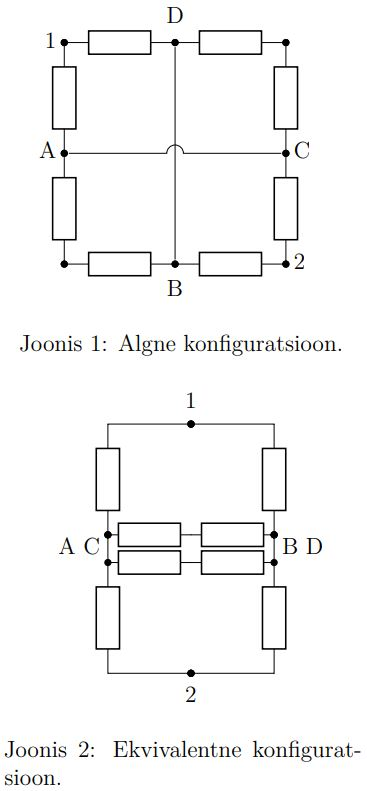
\includegraphics[width=0.28\textwidth]{2020-v2g-04-yl.jpg}
	\vspace{-40pt}
\end{wrapfigure}
Tähistame joonisel punktid A, B, C
ja D. Paneme tähele, et kuna
A ja C on ühendatud omavahel
juhtmega, mille takistuse võime
lugeda nulliks, siis A = C \pp{1}. Samal
põhjusel B = D \pp{1}. Nüüd võime
skeemi ümber joonistada nii, nagu
näidatud joonisel 2. \pp{2}

Sümmeetria tõttu ei läbi punktide A, C ja B, D vahelist silda kunagi vool \pp{2}, seega lihtsustub skeem
kujule, kus on vaid neli ülejäänud takistit \pp{1}, mille kogutakistuseks tuleb $\frac{2R}{2} = R$ \pp{1}
\probend